\scanpage{237}

Dans ces conditions

(i) Le système projectif $(\underline{\pi}_0(G_n))_n$ est essentiellement constant.

(ii) Les systèmes $(G_n^0)_n$ (donc aussi le système $(G_n)$) \unsure{satisfont|satisfait} (M.L.).

(iii) \deleted{P\unsure{our} \illegible{3}} \deleted{(\unsure{s.c.} \unsure{est nulle})} $\exists n_0$ tq \deleted{et conoyau} que \unsure{pour|$\forall$} $m\geq n\geq n_0$, le \unsure{conoyau|noyau} de $G_m\longrightarrow G_n$ soit un groupe vectoriel \deleted{sans torsion (donc} en car $=0$, et \deleted{\unsure{purement}} radiciel en car. $>0$.

\deleted{\unsure{en} \illegible{2} $\unsure{\operatorname{car}>0}$}

\inserted{Si la car. est nulle et si les \deleted{\unsure{connexes}} $\operatorname{Ker}(G_{n+1}\rightarrow G_n)$ sont unipotents, alors les noyaux des $(\unsure{G_m\rightarrow G_n})$ sont aussi vectoriels.}

\uline{Corollaire 2} Supposons que les $\operatorname{Ker}(G_m\rightarrow G_n)$ \inserted{\figure{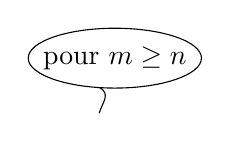
\begin{tikzpicture}[baseline=-.5ex]\draw (0,0) ellipse (1.1 and .38);\node at (0,0) {pour $m\geq n$};\draw (-.2,-.37)..controls(-.05,-.45)and(-.15,-.55)..(-.2,-.7);\end{tikzpicture}}} soient \deleted{$=$}\inserted{de} plus des groupes \deleted{\unsure{commut.} vectoriels} linéaires \deleted{\unsure{résolubles}}\inserted{\figure{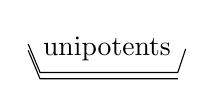
\begin{tikzpicture}[baseline=-.5ex]\node at (0,0) {unipotents};\draw (-1,.06)--(-.85,-.3)--(.9,-.3)--(1,0);\draw (-1,-.02)--(-.85,-.38)--(.9,-.38);\end{tikzpicture}}}, \deleted{supposons $k$ parfait} et supposons $k$ parfait [le cas important est $k$ de car. 0] Alors le système des $(G_n(k))_n$ satisfait ML

\mspage{236}
